\chapter{EFT-Modell mit MadGraph5}
In diesem Kapitel erfolgt eine Variation der Wilson-Koeffizienten mit Hilfe  von MadGraph5 unter der Verwendung eines EFT-Modells. Dies ermöglicht die Berechnung eines approximierten Modells der Wirkungsquerschnitte für den EFT\textit{fitter} mit dessen Hilfe die Wilson-Koeffizienten bestimmt werden können. Dieses approximierte Modell wird benötigt, um die Laufzeiten des EFT\textit{fitter} zu verringern.

\section{Wirkungsquerschnitt}
Der Fit des EFT\textit{fitter}s basiert auf einem funktionellen Zusammenhang zwischen den Observablen, in diesem Fall den Wirkungsquerschnitten, und den Operatoren höherer Ordnung. Diese Abhängigkeit wird durch das implementierte Modell in einer Likelihood ausgedrückt. Diese Likelihood wird mit einer Approximation durch MG bestimmt, da die Laufzeit des EFT\textit{fitter}s dadurch deutlich geringer wird.\\
Für die Berechnung des Wirkungsquerschnitts werden die zugehörigen Feynman-Graphen, sowohl die des SM, als auch die der EFT-Operatoren, betrachtet. Damit ergibt sich die Approximation des Wirkungsquerschnittes zu:
\begin{align}
  \sigma = \sigma_{SM} + \frac{1}{\Lambda^2} \sum_{i} C_i \sigma_i^\text{interf.} + \frac{1}{\Lambda^4} \sum_{i \leq j} C_i C_j \sigma_{ij}^\text{BSM} + \mathcal{O} \left(\frac{1}{\Lambda^6}\right).
\end{align}
Die einzelnen Wirkungsquerschnitte $\sigma$ besitzen eine quadratische Abhängigkeit von den Wilson-Koeffizienten $C_i$ und die BSM-Beiträge in führender Ordnung ergeben sich durch die Interferenz zwischen dem SM und der BSM-Physik. Dies liegt unter anderem daran, dass die Beiträge durch die BSM-Physik-Beiträge alleine mit $\frac{1}{\Lambda^4}$ unterdrückt sind. Untersuchungen~\cite{Fichet:2016iuo} haben ergeben, dass diese Beiträge trotzdem betrachtet werden sollten, um ein Modell für die Abhängigkeit der Wirkungsquerschnitte von den Wilson-Koeffizienten zu erhalten, da sie zur Genauigkeit des Modells beitragen.

\section{Variation der Wilson-Koeffizienten in MadGraph5}%
%
Zur Bestimmung dieses Modells ist es notwendig, die Wirkungsquerschnitte für verschiedene Konfigurationen der Wilson-Koeffizienten zu bestimmen, um sowohl den Einfluss einzelner als auch mehrerer Operatoren untersuchen zu können.
Eine Möglichkeit die Wilson-Koeffizienten zu variieren, ist mit Hilfe eines  EFT-Modells für MG, das Operatoren der Massendimension sechs enthält und damit eine Berechnung der Wirkungsquerschnitte unter dem Einfluss dieser Operatoren ermöglicht. Dazu wird in MG das TEFT\_EF UFO Modell~\mcite{Bylund:2016phk, Franzosi:2015osa, Zhang:2016omx, Degrande:2011ua} eingebunden.
Dies enthält einige der für die Top-Quark-Physik relevanten Operatoren der Dimension sechs und insbesondere die, die an dem Prozess $pp~\rightarrow~t\bar{t}~\gamma$ beteiligt sind.
Die Berechnung erfolgt mit dem genannten Modell in NLO in QCD unter der Verwendung des $\text{CTEQ}6\text{L}1$ PDF-Satzes.
Zudem wird die BSM-Energieskala auf $\Lambda = \SI{1}{\tera\electronvolt}$ festgelegt.
Unter diesen Vorraussetzungen wird der Prozess $pp~\rightarrow~t\bar{t}~\gamma$ mit den von ATLAS genutzten Schnitten für den gemessenen Phasenraum implementiert.\\
Die berechneten Monte-Carlo-Wirkungsquerschnitte:
\begin{align}
  \sigma_{MC}({C_i}) = \sigma_{SM} + \sum_{i} C_i \frac{\sigma_i}{\Lambda^2} + \sum_{i \leq j} C_i C_j \frac{\sigma_{ij}}{\Lambda^4} + \mathcal{O}\left(\frac{1}{\Lambda^6}\right)
\end{align}
bilden die Stützstellen zur späteren Bestimmung der gesuchten Parameter $\sigma_i$ und $\sigma_{ij}$.
Mit Hilfe des Vakuumerwartungswerts des Higgs-Feldes $v = \SI{246}{\giga\electronvolt}$ und der Wahl $\Lambda = \SI{1}{\tera\electronvolt}$ lassen sich die $\sigma_{MC}$ in die Größenordnung einer Kopplungsstärke umrechnen.
Unter Vernachlässigung von Termen der Ordnung $\mathcal{O}(\frac{1}{\Lambda^6})$, ergeben sie sich zu:
\begin{align}
  \sigma_{MC}({\tilde{C_i}}) \approx \sigma_{SM} + \sum_{i} \tilde{C_i} \bar{\sigma_i} + \sum_{i \leq j} \tilde{C_i} \tilde{C_j} \bar{\sigma}_{ij}.
\end{align}
Hierbei sind die $\tilde{C}_i = \frac{v^2}{\Lambda^2} C_i$, $\bar{\sigma}_i = \frac{\sigma_i}{v^2}$ und $\bar{\sigma}_{ij} = \frac{\sigma_{ij}}{v^4}$ die zugehörgen Parameter.
Bei der Berechnung des $t\bar{t}\gamma$ Produktionswirkungsquerschnitts können, wie in Kapitel~\ref{top} bereits erwähnt, die Operatoren $O_{tG}$, $O_{tW}$ und $O_{tB}$ beitragen. Damit ergibt sich die Interpolationsfunktion zu:
\begin{align}
  \sigma_{t\bar{t}\gamma, MC}({\tilde{C}_{tG}, \tilde{C}_{tW}, \tilde{C}_{tB}}) = \sigma_{SM} + \tilde{C}_{tG}\bar{\sigma}_{tG} + \tilde{C}_{tW}\bar{\sigma}_{tW} + \tilde{C}_{tB}\bar{\sigma}_{tB}\\ \nonumber
  + \tilde{C}_{tG}^2\bar{\sigma}_{tGtG} + \tilde{C}_{tW}^2\bar{\sigma}_{tWtW} + \tilde{C}_{tB}^2\bar{\sigma}_{tBtB}\\
  + \tilde{C}_{tG} \tilde{C}_{tW}\bar{\sigma}_{tGtW} + \tilde{C}_{tG} \tilde{C}_{tB}\bar{\sigma}_{tGtB} + \tilde{C}_{tW} \tilde{C}_{tB}\bar{\sigma}_{tWtB} \nonumber
\end{align}
und es müssen insgesamt zehn Parameter $\bar{\sigma_i}$ und $\bar{\sigma}_{ij}$ bestimmt werden. Dazu werden die Wilson-Koeffizienten $C_{tG}$, $C_{tW}$ und $C_{tB}$ im Bereich $[-30~,~30]$ variiert. Auf Grund der statistischen Unsicherheiten werden insgesamt $50$ verschiedene Variationen durchgeführt, bei denen ein, zwei oder alle der Wilson-Koeffizienten ungleich Null sind.
Um erneut nur die Lepton+Jets-Endzustände zu betrachten, müssen auch in diesem Fall die $\sigma_{t\bar{t}\gamma, MC}$ mit dem Verzweigungsverhältnis für Lepton+Jets-Ereignisse $\mathrm{BR} \approx \SI{30}{\percent}$ multipliziert werden.
Aus diesen Berechnungen lassen sich dann mit der Methode der kleinsten Quadrate die gesuchten Parameter bestimmen, aus denen sich schließlich das Modell für den EFT\textit{fitter} ergibt.


\section{Bestimmung des Modells für den EFT\textit{fitter}}
\label{Modell}
Durch die Bestimmung der gesuchten Parameter mit der Methode der kleinsten Quadrate werden die folgenden Wirkungsquerschnitte bestimmt:
\begin{table}[H]
    \centering
   \begin{tabular}{ll}
     $\sigma_{SM}   = \SI{202.19}{\femto\barn\per\giga\electronvolt\squared} $  & $\bar{\sigma}_{tW}   = \SI{21.7}{\femto\barn\per\giga\electronvolt\squared}$\\
     $\bar{\sigma}_{tB}   = \SI{21.7}{\femto\barn\per\giga\electronvolt\squared}$    & $\bar{\sigma}_{tG}   = \SI{761.4}{\femto\barn\per\giga\electronvolt\squared}$\\
     $\bar{\sigma}_{tWtW} = \SI{11.7}{\femto\barn\per\giga\electronvolt\tothe{4}}$    & $\bar{\sigma}_{tBtB} = \SI{11.8}{\femto\barn\per\giga\electronvolt\tothe{4}}$\\
     $\bar{\sigma}_{tGtG} = \SI{48.4}{\femto\barn\per\giga\electronvolt\tothe{4}}$    & $\bar{\sigma}_{tGtW} = \SI{6863.8}{\femto\barn\per\giga\electronvolt\tothe{4}}$\\
     $\bar{\sigma}_{tGtB} = \SI{-6483.3}{\femto\barn\per\giga\electronvolt\tothe{4}}$ & $\bar{\sigma}_{tWtB} = \SI{279.2}{\femto\barn\per\giga\electronvolt\tothe{4}}$
   \end{tabular}
\end{table}
Die Unsicherheiten aus dem Fit mit der Methode der kleinsten Quadrate werden hier vernachlässigt, da diese nicht im Modell des EFT\textit{fitter}s implementiert werden können. Die gültigen Stellen orientieren sich an der Fehlern, der berechneten Stützstellen.\\
In den Abbildungen~\ref{fig:tp} und~\ref{fig:WtG} ist erkennbar, dass der Fit die erwartete quadratische Form in den jeweiligen Parametern aufweist. Die für die beiden Wilson-Koeffizienten $\tilde{C}_{tW}$ und $\tilde{C}_{tB}$ berechneten Wirkungsquerschnitte folgen dem erwarteten parabelförmigen Verlauf, wie in Abbildung~\ref{fig:WtW} und~\ref{fig:WtB} veranschaulicht. Die beiden Wilson-Koeffizienten, die zu den beiden an der Photonabstrahlung beteiligten Operatoren gehören, tragen gleich bei. Dies war zuerwarten, da theoretische Berechnungen bewiesen haben, dass die beiden Operatoren $\tilde{O}_{tW}$ und $\tilde{O}_{tB}$ ununterscheidbar sind~\cite{Bylund:2016phk}. Lediglich die berechneten Wirkungsquerschnitte für den Wilson-Koeffizienten $\tilde{C}_{tG}$ weisen teilweise Abweichungen von dem parabelförmigen Verlauf auf, wie in Abbildung~\ref{fig:WtG} erkennbar ist. Zudem fällt auf, dass der Wertebreich der Wirkungsquerschnitte deutlich höher ist, als bei den Wilson-Koeffizienten $\tilde{C}_{tW}$ und $\tilde{C}_{tB}$.\\
Der Fit für den Wilson-Koeffizienten $\tilde{C}_{tG}$ in Abbildung~\ref{fig:WtG} könnte verbessert werden, indem mehr Stützstellen berechnet werden.\\
\begin{figure}
  \begin{subfigure}[c]{0.5\textwidth}
    \centering
    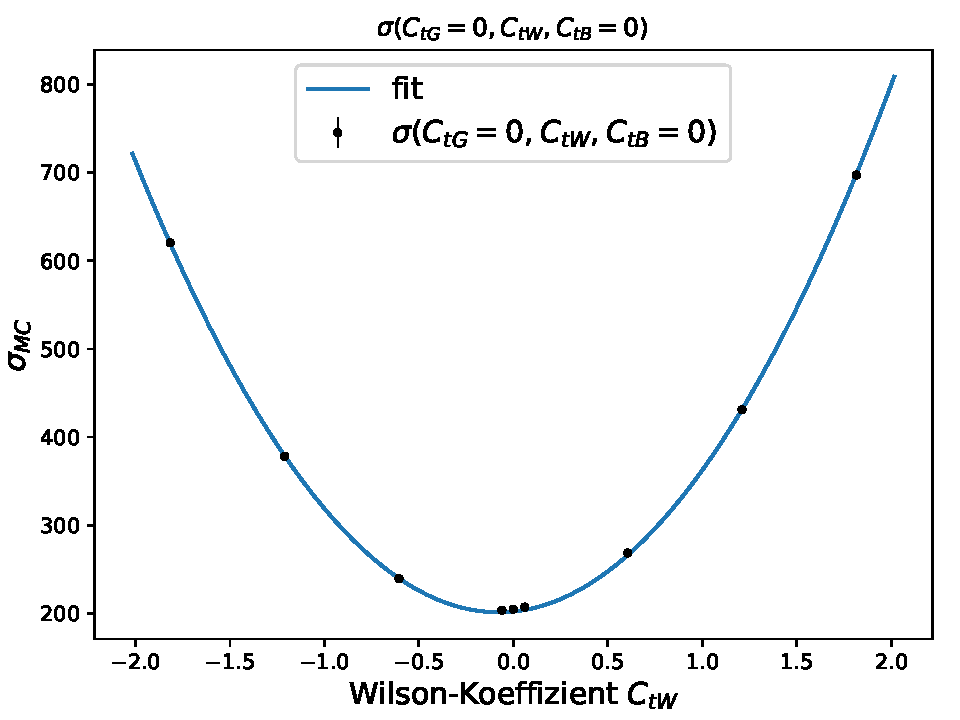
\includegraphics[width=\textwidth]{Plots/combi_plot_tW.pdf}
    \subcaption{Verlauf für $\tilde{C}_{tW}$ mit $\tilde{C}_{tB}=\tilde{C}_{tG}=0$.}
    \label{fig:WtW}
  \end{subfigure}
  \begin{subfigure}[c]{0.5\textwidth}
    \centering
    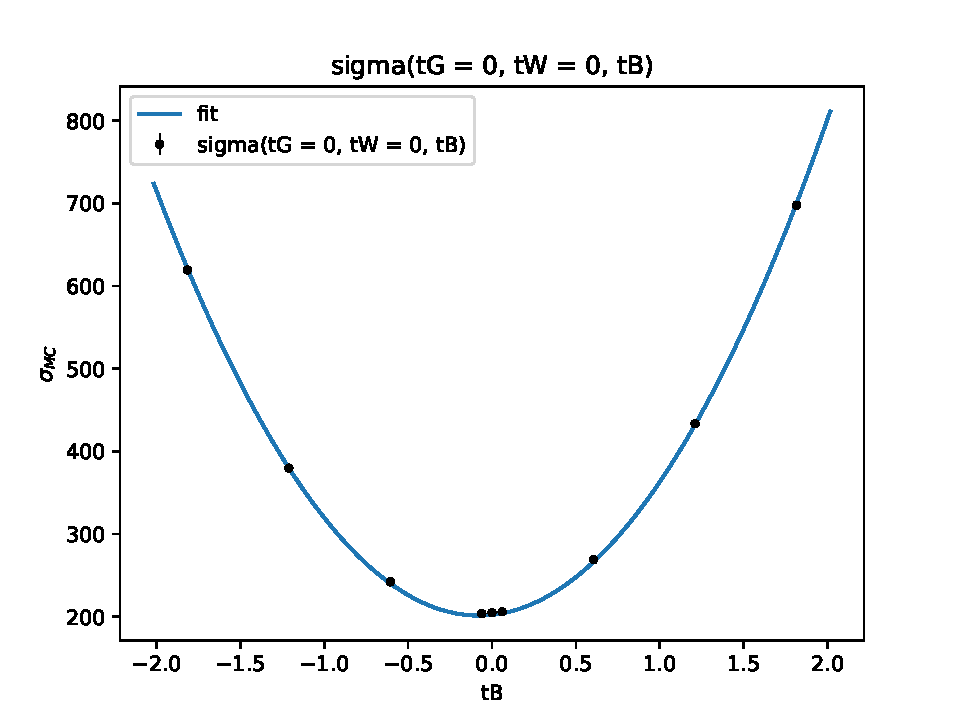
\includegraphics[width=\textwidth]{Plots/combi_plot_tB.pdf}
    \subcaption{Verlauf für $\tilde{C}_{tB}$ mit $\tilde{C}_{tW}=\tilde{C}_{tG}=0$.}
    \label{fig:WtB}
  \end{subfigure}
  \caption{Graphische Darstellung des parabelförmigen Verlaufs der Wirkungsquerschnitte für die Betrachtung einzelner Wilson-Koeffizienten.}
  \label{fig:tp}
\end{figure}
\begin{figure}
  \centering
  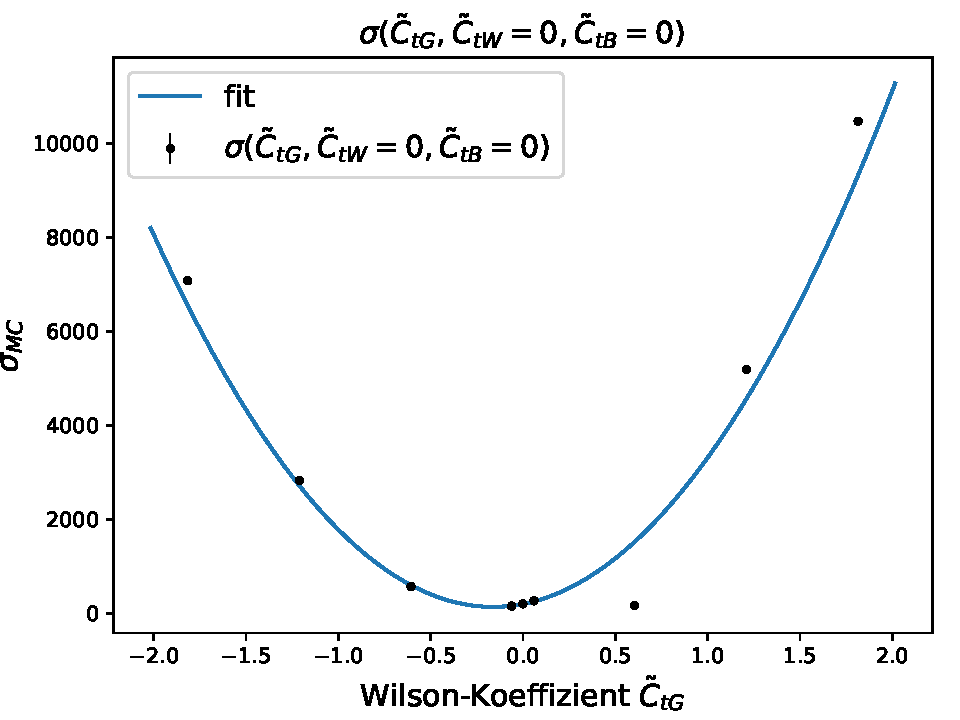
\includegraphics[width=0.6\textwidth]{Plots/combi_plot_tG.pdf}
  \caption{Graphische Darstellung des parabelförmigen Verlaufs der Wirkungsquerschnitte für den Wilson-Koeffizienten $\tilde{C}_{tG}$, wenn $\tilde{C}_{tW}=\tilde{C}_{tB}=0$ gilt.}
  \label{fig:WtG}
\end{figure}
%
%
\chapter{EFT-Interpretation des \texorpdfstring {$t\bar{t}\gamma$}{math}-Produktionswirkungsquerschnitts}
In diesem Kapitel erfolgt die Untersuchung der am $t\bar{t}\gamma$-Produktionswirkungsquerschnitt beteiligten Wilson-Koeffizienten mit dem EFT\textit{fitter}. Dazu wird das mit MadGraph bestimmte Modell aus Kapitel~\ref{Modell} im EFT\textit{fitter} implemeniert und mit Hilfe der ATLAS-Messung die Wilson-Koeffizienten eingeschränkt.

\section{Einschränkung der Wilson-Koeffizienten}
 Der von ATLAS gemessene $t\bar{t}\gamma$-Produktionswirkungsquerschnitt kann mit Hilfe des EFT\textit{fitter} auf mögliche Abweichungen durch die EFT-Operatoren $O_{tG}$, $O_{tW}$ und $O_{tB}$ getestet werden. Dazu wird das in Kapitel~\ref{Modell} berechnete Modell verwendet. Es ermöglicht Einschränkungen für die Wilson-Koeffizienten der EFT-Operatoren zu finden.
In den Abbildungen~\ref{fig:ctw},~\ref{fig:ctb} und~\ref{fig:ctg} sind die marginalisierten, eindimensionalen Posteriorverteilung der Wilson-Koeffizienten, die mit Hilfe des EFT\textit{fitter}s berechnet wurden, dargestellt.
Da der Fit mit einem quadratischen Modell in den Wilson-Koeffizienten durchgeführt wird, stimmt die Messung an zwei Stellen mit der Vorhersage überein, sodass sich zwei Peaks ergeben.
Da für jeden Wilson-Koeffizienten eines der Maxima in der Nähe von Null liegt und das kleinste $\SI{68.1}{\percent}$-Intervall diesen Wert umfasst, kann die SM Vorhersage, dass die Wilson-Koeffizienten Null sind, nicht verworfen werden.
Das $\SI{68.1}{\percent}$-Intervall ist für alle Wilson-Koeffizient in Abbildung~\ref{fig:wil} dargestellt. Auffällig ist, dass die Intervalle alle die Null enthalten, aber nur $\tilde{C}_{tG}$ um diese zentriert ist und zudem die Einschränkung deutlich kleiner ist.
Dies liegt an den größeren Werten der Wirkungsquerschnitte, die bereits in Abbildung~\ref{fig:WtG} beobachtet wurden. Da bei kleinen Werten des Wilson-Koeffizeinten der Wirkungsquerschnitt sehr groß wird, ist das $1\sigma$-Intervall schnell nicht mehr mit der Messung verträglich.
Zudem ist zu beobachten, dass die Einschränkungen für $\tilde{C}_{tW}$ und $\tilde{C}_{tB}$ nahezu übereinstimmen, dies liegt, wie bereits in Kapitel~\ref{Modell} erwähnt, an der Ununterseidbarkeit der beiden Operatoren $\tilde{O}_{tW}$ und $\tilde{O}_{tB}$.
Die noch relativ großen Intervalle für die Einschränkung von $\tilde{C}_{tW}$ und $\tilde{C}_{tB}$ motivieren eine Kombination mit weiteren Observablen zum Beipiel dem $t\bar{t}Z$-Produktionswirkungsquerschnitt, der sensitiv auf die gleichen Operatoren ist. So kann eine bessere Einschränkung erfolgen und unter Umständen eines der beiden Maxima ausgeschlossen werden, sodass sich das $\SI{68.1}{\percent}$-Intervall verkleinert.
Um eine höhere Aussagekraft dieser Ergebnisse zu erhalten, empfielt es sich die Einschränkung mit mehreren Messungen für den $t\bar{t}\gamma$-Produktionswirkungsquerschnitt im gleichen Phasenraum zu berechnen.
\begin{figure}
    \centering
    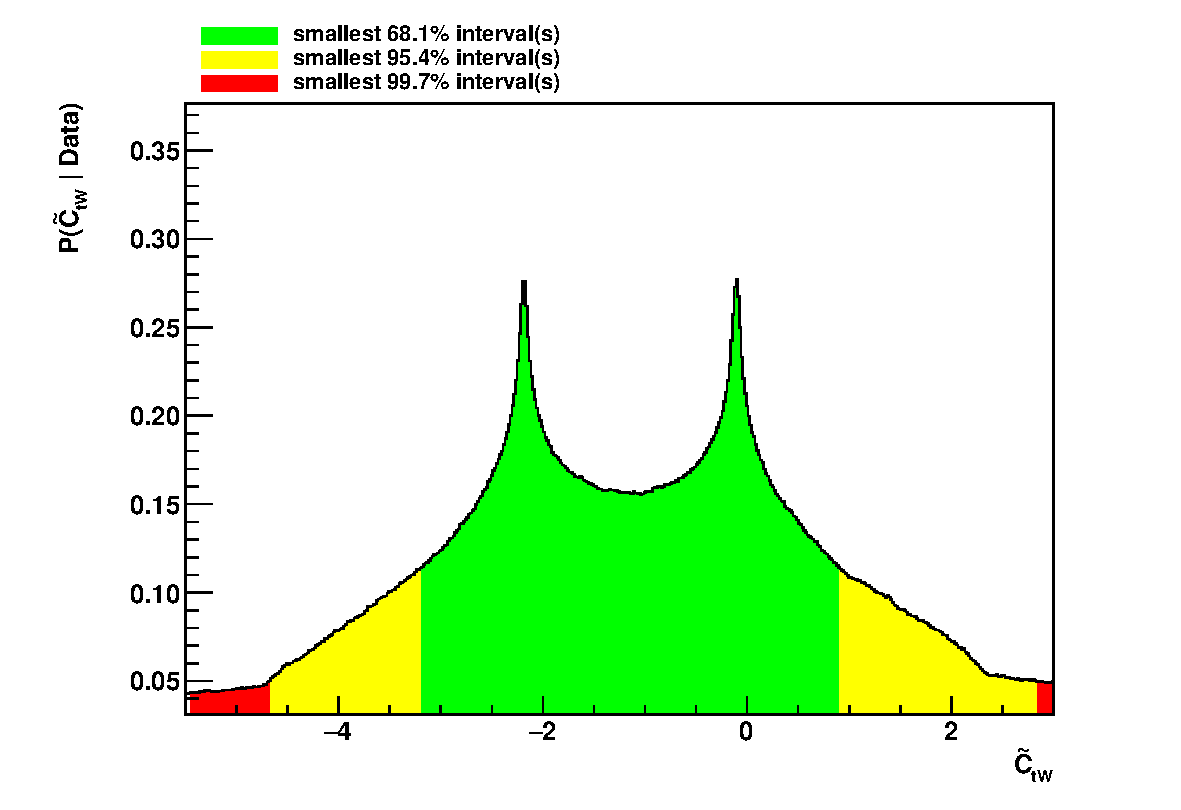
\includegraphics[width=0.8\textwidth]{Plots/ctw.pdf}
    \caption{Eindimensionale Posteriorverteilung des Wilson-Koeffizienten $\tilde{C}_{tW}$.}
    \label{fig:ctw}
\end{figure}
\begin{figure}
    \centering
    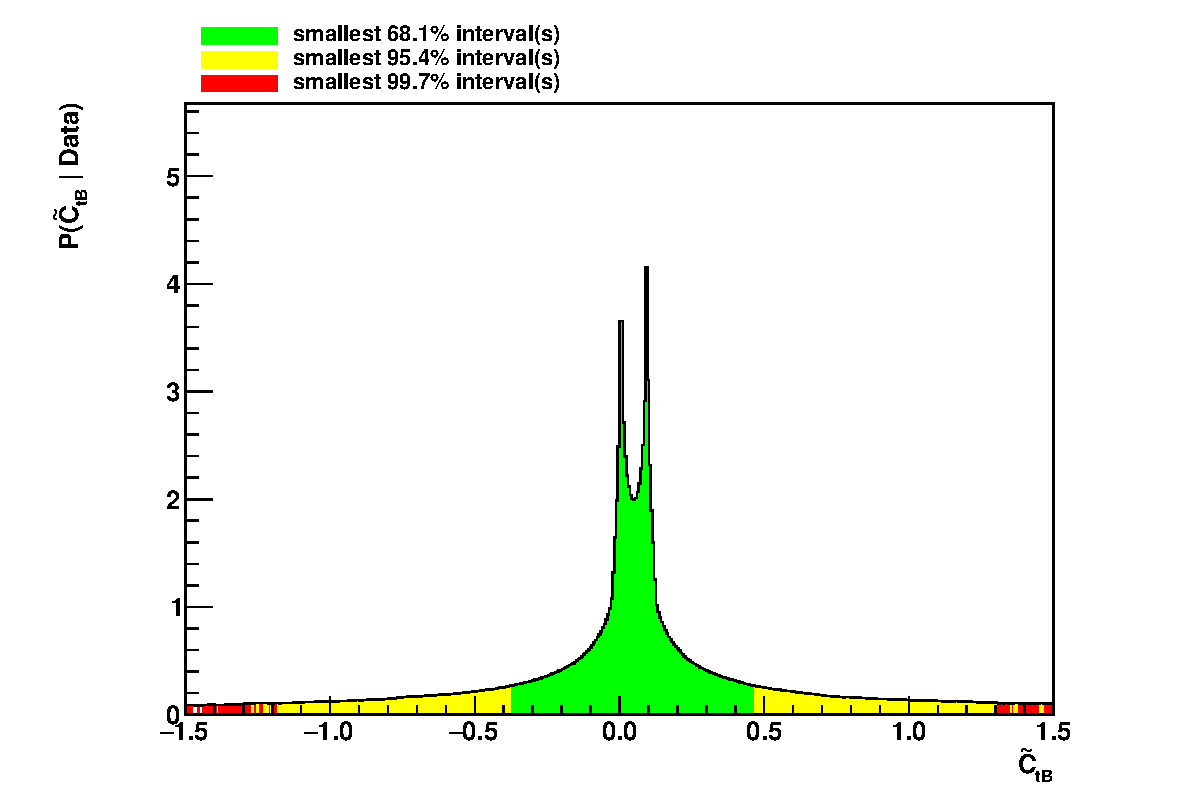
\includegraphics[width=0.8\textwidth]{Plots/ctb.pdf}
    \caption{Eindimensionale Posteriorverteilung des Wilson-Koeffizienten $\tilde{C}_{tB}$.}
    \label{fig:ctb}
\end{figure}
\begin{figure}
    \centering
    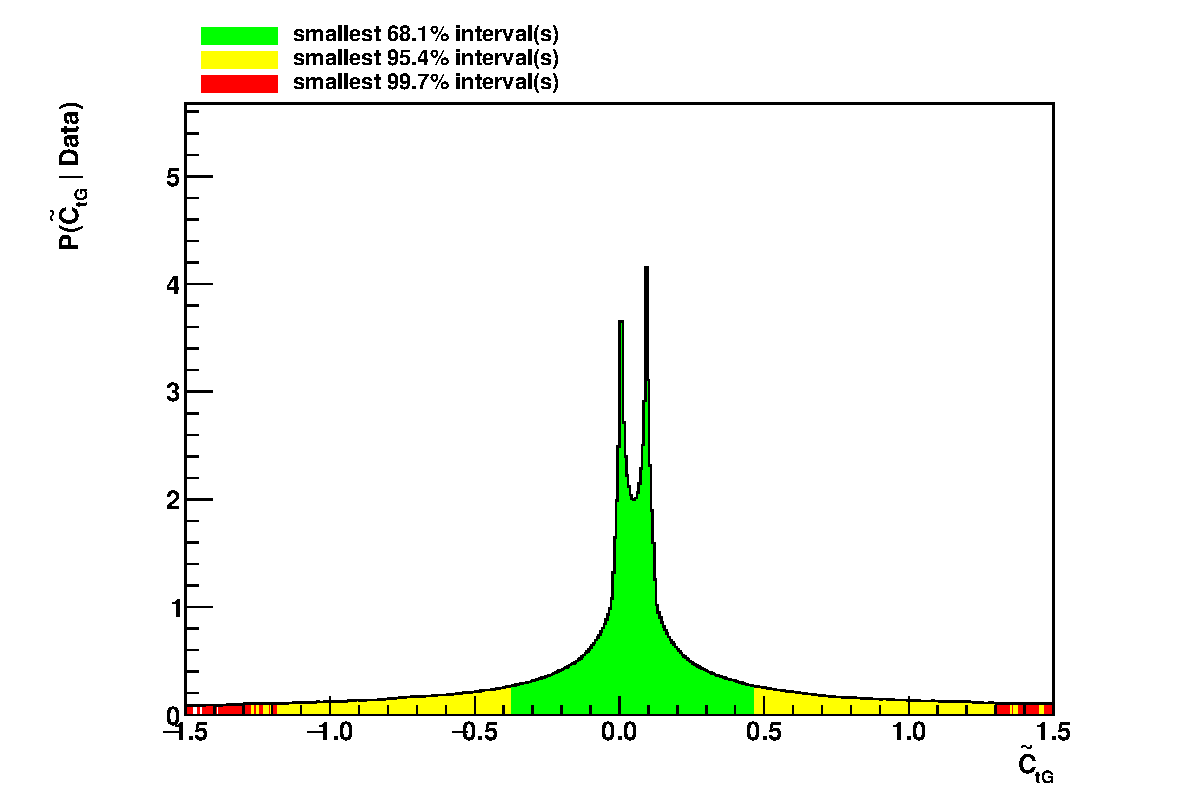
\includegraphics[width=0.8\textwidth]{Plots/ctg.pdf}
    \caption{Eindimensionale Posteriorverteilung des Wilson-Koeffizienten $\tilde{C}_{tG}$.}
    \label{fig:ctg}
\end{figure}
\begin{figure}
    \centering
    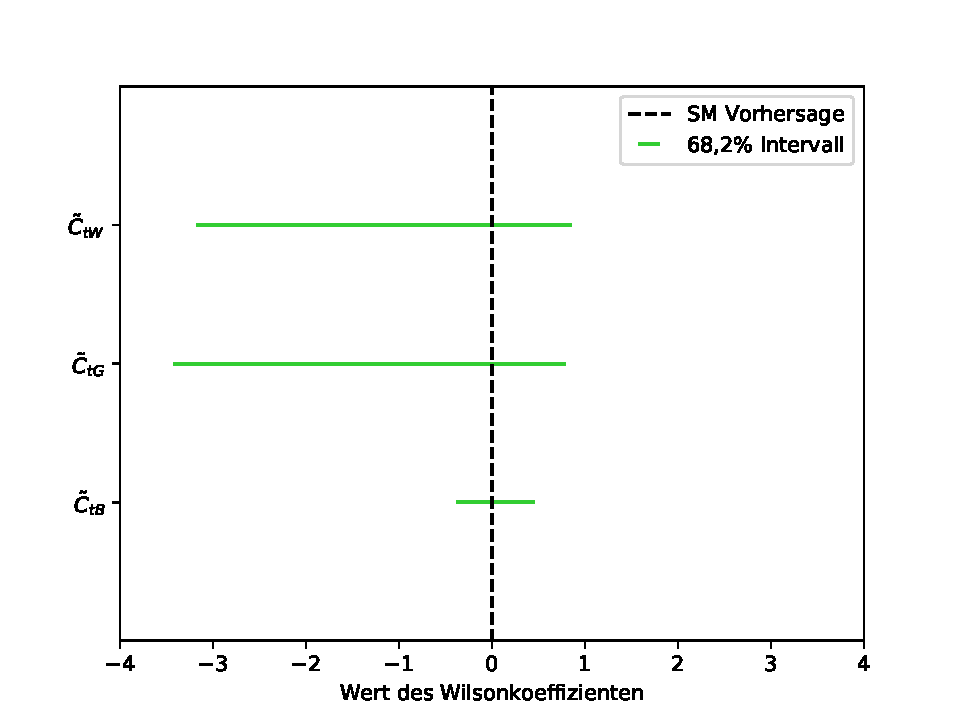
\includegraphics[width=0.7\textwidth]{Plots/wilson.pdf}
    \caption{Darstellung des kleinsten $\SI{68.1}{\percent}$ Intervalls der Wilson-Koeffizienten zur Veranschaulichung der Verträglichkeit mit Null.}
    \label{fig:wil}
\end{figure}
%
%
\chapter{Zusammenfassung}
Ein Bereich der aktueller Forschung in der Teilchenphysik liegt in der BSM-Physik, diese ist dadurch motiviert, dass verschiedene Effekte nicht mit dem Standardmodell zu erklären sind. Eine Möglichkeit diese Effekte zu beschreiben, bieten modellunabhänigige effektive Feldtheorien. Ihre Vorteile sind, dass auch Teilchen, die an aktuellen Beschleunigern nicht produziert werden können, mit ihnen beschrieben werden können. Die Untersuchung des Top-Quarks im Zusammenhang von EFT ist dadurch motiviert, dass verschiedene Faktoren, wie beispielsweise die Yukawa-Kopplung des Top-Quarks, dafür sprechen, dass dieses stark an BSM-Physik koppeln könnte. \\
Im Rahmen dieser Arbeit erfolgte eine Interpretation von $t\bar{t}\gamma$-Messungen in Bezug auf EFT. Zunächst wurde eine Phasenraumstudie durchgeführt, um die in unterschiedlichen fiducial Phasenräumen durchgeführten ATLAS- und CMS-Messungen zu kombinieren. Dazu wurde ein Faktor zwischen den Phasenräumen bestimmt und auf die CMS-Messungen angewendet. Die anschließende Kombination der Messungen, unter der Annahme, dass diese unkorreliert seien, lieferte:
\begin{align*}
  \sigma_{\text{Kombi}} = 150 \pm 18~ \si{\femto\barn}.
\end{align*}
Es fiel auf, dass das kombinierte Ergebnis sehr nah an dem ATLAS-Messwert lag. Daher lässt sich sagen, dass eine Kombination von Messungen nur sinnvoll ist, wenn sie im identischen oder nahezu gleichem Phasenraum durchgeführt wurden. Dies liegt vor allem an dem Einfluss der Unsicherheiten auf das Ergegnis einer Kombination. Im Anschluss erfolgte eine Korrelationsstudie, um den Einfluss einer möglichen Korrelation zwischen den Unsicherheiten der Messungen auf das Ergebnis der Kombination zu untersuchen. Dabei ergibt sich, dass die Kombination stark von einer möglichen Korrelation abhängt, sodass diese zunächst untersucht werden sollte.
Im zweiten Teil dieser Arbeit erfolte die EFT-Interpretation des $t\bar{t}\gamma$-Produktionswirkungsquerschnitts mit dem EFT\textit{fitter}. Dafür wurden die Wilson-Koeffizienten $C_{tG}$, $C_{tW}$ und $C_{tB}$, der am Produktionswirkungsquerschnitt beteiligten Operatoren, untersucht. Innerhalb des kleinsten $\SI{68.1}{\percent}$-Intervalls sind alle drei Wilson-Koeffizienten mit Null verträglich. Die Intervalle, der an der Photonabstrahlung beteiligten Wilson-Koeffizienten $C_{tW}$ und $C_{tB}$, sind jedoch relativ breit.\\
Dies motiviert eine Untersuchung dieser Wilson-Koeffizienten mit weiteren Messungen, wie beispielsweise der $t\bar{t}\gamma$-Produktionswirkungsquerschnitt, bei denen die entsprechenden BSM-Operatoren beteiligt sind. Dabei könnte sich eine Inkompatibilität mit Null ergeben und somit die Existenz der Operatoren $O_{tW}$ und $O_{tB}$ beweisen.
